% Preamble
\documentclass{article}

% Packages
\usepackage{docmute} % LaTeX 合并独立子文件
\usepackage{amsmath} % Advanced math typesetting
\usepackage[utf8]{inputenc} % Unicode support (Umlauts etc.)
\usepackage[ngerman]{babel} % Change hyphenation rules
\usepackage{hyperref} % Add a link to your document
\usepackage{graphicx} % Add pictures to your document
\usepackage{listings} % Source code formatting and highlighting
\usepackage{booktabs}
\usepackage[backend=bibtex,style=verbose-trad2]{biblatex} % Use biblatex package
\usepackage{xcolor} % add color to text


\bibliography{quick} % The name of the .bib file (name without .bib)

% Main document
\begin{document} % Set up the maketitle command
\author{Massyao Tse}
\title{Learning \LaTeX{}}
\date{\today{}} % You can remove \today{} and type a date manually

\maketitle{} % Generates title

\tableofcontents{} % Generates table of contents from sections

% --------------------------------
% -------  chapter 1  ------------
% --------------------------------
\maketitle
\newpage
\section{How to use \LaTeX{}}
This is a quick introduction to the most common features of \LaTeX{}. For more features, check the other lessons on \url{http://www.latex-tutorial.com} and the articles on \url{http://blog.latex-tutorial.com}. 
\subsection{Document structure}
The documents in \LaTeX{} are structured slightly different from Word. The document consists of two parts, the preamble and the main document. If you're familiar with programming, then you might want to compare the structure with that of a C/C++ file.

\subsubsection{Preamble}
The purpose of the preamble is to tell \LaTeX{} what kind of document you will set up and what packages you are going to need. A package is a set of additional functions such as \emph{amsmath} for additional math formatting. For this document, the preamble looks like this:

\begin{lstlisting}[language={[LaTeX]TeX},caption=Preamble of this document,breaklines=true,frame=single]
% Preamble
% ---
\documentclass{article}

% Packages
% ---
\usepackage{amsmath} % Advanced math typesetting
\usepackage[utf8]{inputenc} % Unicode support (Umlauts etc.)
\usepackage[ngerman]{babel} % Change hyphenation rules
\usepackage{hyperref} % Add a link to your document
\usepackage{graphicx} % Add pictures to your document
\usepackage{listings} % Source code formatting and highlighting
\end{lstlisting}

You can set the class of the documentclass with the \emph{documentclass} command and add packages with the \emph{usepackage} command. Only the \emph{documentclass} command is mandatory, you can compile a document also without packages, yet some functions may be missing in this case. The \emph{usepackage} command \emph{must not} be used in the main document.

\subsubsection{Main document}
The main document is contained within the \emph{document} environment like this:

\begin{lstlisting}[language={[LaTeX]TeX},caption=Main part of a \LaTeX{} document.,breaklines=true,frame=single,frame=single]
\begin{document}
% ...
% ... Text goes here
% ...
\end{document}
\end{lstlisting}

Within those two statements, we can add the content of our document. But just adding the text is probably not enough, since we also have to apply formatting to it.

\subsection{Formatting in \LaTeX{}}
Formatting in \LaTeX{} can be applied by the use of commands and environment. The topmost environment is the document environment as described in Listing ref{lst:main}. So there are obviously more environments, but how to find them? Well the easiest way is to download a \LaTeX{} cheat sheet which provides a list of the most useful commands and environments. For most packages there is also a manual available, which can be found on Google.

\subsubsection{Math typesetting}
To introduce you to math typesetting and environments, I will demonstrate you how to format some simple equations:

\begin{align}
f(x) &= x^2\\
f'(x) &= 2x\\
F(x) &= \int^a_b f(x)dx\\
F(x) &= \frac{1}{3}x^3\\
M(A) &= \left[
    \begin{matrix}
    f(x) & g(x)\\
    f'(x) & g'(x)
    \end{matrix}
    \right]\\
H(f) &= \int\left\{\frac{\lambda}{\sqrt{x}}\right\}^3dx
\end{align}



This can be done with the following code:

\begin{lstlisting}[language={[LaTeX]TeX},caption=Typesetting equations in \LaTeX{}.,breaklines=true,frame=single]
\begin{align}
f(x) &= x^2\\
f'(x) &= 2x\\
F(x) &= \int f(x)dx\\
F(x) &= \frac{1}{3}x^3
\end{align}
\end{lstlisting}

As you can see, we again have a \emph{begin} and \emph{end} statement, this it's applying the \emph{align} environment. This will align the equations at the ampersand (\&) sign. Naturally, those will be placed in front of the equality sign. If you watched carefully, you will see that \LaTeX{} magically added sequential numbers to all equations. \LaTeX{} does this for many other elements too. More about that in the next chapter.

\subsubsection{Document layout}
Usually a document does not only consist of a bunch of equations, but needs some kind of structure too. We are usually going to need at least:

\begin{itemize}
\item{Title/Titlepage}
\item{Table of contents}
\item{Headlines/Sections}
\item{Bibliography}
\end{itemize}

\LaTeX{} provides all the commands we need. The following commands will help us:\\

\begin{lstlisting}[language={[LaTeX]TeX},caption=Useful commands to structure a document.,label=lst:main,breaklines=true,frame=single]
\section{Text goes here} % On top of document hierarchy; automatically numbered
\subsection{}
\subsubsection{}
\paragraph{} % Paragraphs have no numbering
\subparagraph{}

\author{Claudio Vellage} % The authors name
\title{A quick start to \LaTeX{}} % The title of the document
\date{\today{}} % Sets date you can remove \today{} and type a date manually
\maketitle{} % Generates title
\tableofcontents{} % Generates table of contents from sections and subsections

\\ % Linebreak
\newpage{} % Pagebreak
\end{lstlisting}

There are commands to create sections, the sections are numbered automatically and the \emph{tableofcontents} command will use them to generate the table of contents. You don't have to do it yourself, ever. \LaTeX{} also provides commands to generate the title using the \emph{maketitle} command. This needs the \emph{author}, \emph{title} and \emph{date} command to be set. If you place the \emph{maketitle} or \emph{tableofcontents} command in your document, the Commands will be added at that exact place, so you probably want them in the very beginning of your document. If you want the title to appear on a single page, simply use the \emph{newline} command.

\subsubsection{Adding a picture}

Most documents will also need some kind of picture. Like this:

\begin{figure}
\includegraphics[width=1.0\textwidth]{picture}
\caption{This figure shows the logo of my website.}
\end{figure}

 Adding them is fairly easy:

\begin{lstlisting}[language={[LaTeX]TeX},caption=Adding pictures in \LaTeX{}.,breaklines=true,frame=single]
\begin{figure}
\includegraphics[width=\textwidth]{picture.png}
\caption{This figure shows the logo of my website.}
\end{figure}
\end{lstlisting}

You have to embed the picture within the \emph{figure} environment, then use the \emph{includegraphics} command to select the image. Note that the picture file has to be in the same directory as your .tex file or you specify the path like this:
\begin{lstlisting}[language={[LaTeX]TeX},caption=How to specify a path.,breaklines=true,frame=single]
% ...
\includegraphics[width=\textwidth]{FOLDERNAME/picture.png}
% ...
\end{lstlisting}

It makes sense to manage all your pictures in subfolders if you have many of them.

\subsection{Sourcecode formatting}

Throughout the book I used the \emph{listings} package to format the \LaTeX{} code snippets. You can specify the language for each \emph{lstlistings} block, in this case i used \LaTeX{} of course and added a caption as well as enabled linebreaking:

\begin{lstlisting}[language={[LaTeX]TeX},caption=How to use the listings package.",breaklines=true,frame=single,escapechar=^]
^\textbackslash^begin{lstlisting}[language={[LaTeX]TeX},caption=,breaklines=true,frame=single]
% Source code goes here
^\textbackslash^end{lstlisting}
\end{lstlisting}

The language is specified as \emph{[DIALECT]LANGUAGE}, here \LaTeX{} is dialect of \TeX{}. A list of all programming languages can be obtained from the \emph{listings} package manual, but you can also just try out if it works.

%\subsubsection{References and Bibliography}\label{sec:ref}
\subsubsection{References and Bibliography}
%You can specify labels for all the things that are automatically numbered. If you want to refer to a section of your document, you'd simply use the \emph{label} and \emph{ref} (reference) command. Where the label indicates what you want to refer to and the reference will print the actual number of the element in your document. This will also work interactively in your PDF reader You can try this feature in section \ref{sec:ref}.

\begin{lstlisting}[language={[LaTeX]TeX},caption=Labels and references in \LaTeX{},breaklines=true,frame=single]
\section{}\label{sec:YOURLABEL}
% ...
I've written text in section \ref{sec:YOURLABEL}.
\end{lstlisting}

Papers usually include a lot of references to the great works of other people. In order to properly cite them, we'd want to use the biblatex package. For this purpose we'd simply add the following code to our preamble:

\begin{lstlisting}[language={[LaTeX]TeX},caption=Preamble code to use biblatex.,breaklines=true,frame=single]
\usepackage[backend=bibtex,style=verbose-trad2]{biblatex} % Use biblatex package
\bibliography{FILENAME} % The name of the .bib file (name without .bib)
\end{lstlisting}

All bibliographic information will be stored in the bibliography (.bib) and \emph{must not} be inside of the .tex file An example could look like this:

\begin{lstlisting}[language={[LaTeX]TeX},caption=Example bibliography file.,breaklines=true,frame=single]
@ARTICLE=
{
VELLAGE:1,
AUTHOR="Claudio Vellage",
TITLE="A quick start to \LaTeX{}",
YEAR="2013",
PUBLISHER="",
}
\end{lstlisting}

Now i could add a self reference using the \emph{cite} command:

\begin{lstlisting}[language={[LaTeX]TeX},caption=The cite command.,breaklines=true,frame=single]
This feature works as I described in \cite{VELLAGE:1}.
\end{lstlisting}

The \emph{biblatex} is very smart and wil print autogenerate the bibliography if we want to. We'd usually do this in the end of the document. Simply add

\begin{lstlisting}[language={[LaTeX]TeX},caption=The cite command.,breaklines=true,frame=single]
\printbibliography
\end{lstlisting}

to our document. More examples can be found on the \href{http://www.latex-tutorial.com/lesson7/}{website}.

\subsubsection{Code}

  \lstdefinestyle{lfonts}{
    basicstyle   = \footnotesize\ttfamily,
    stringstyle  = \color{purple},
    keywordstyle = \color{blue!60!black}\bfseries,
    commentstyle = \color{olive}\scshape,
  }
  \lstdefinestyle{lnumbers}{
    numbers     = left,
    numberstyle = \tiny,
    numbersep   = 1em,
    firstnumber = 1,
    stepnumber  = 1,
  }
  \lstdefinestyle{llayout}{
    breaklines       = true,
    tabsize          = 2,
    columns          = flexible,
  }
  \lstdefinestyle{lgeometry}{
    xleftmargin      = 20pt,
    xrightmargin     = 0pt,
    frame            = tb,
    framesep         = \fboxsep,
    framexleftmargin = 20pt,
  }
  \lstdefinestyle{lgeneral}{
    style = lfonts,
    style = lnumbers,
    style = llayout,
    style = lgeometry,
  }
  \lstdefinestyle{python}{
      language = {Python},
      style    = lgeneral,
  }

  \lstinline[style = python]|print('Hello world!')|
  \begin{lstlisting}[style = python]
  for x in range(101):
      print('fizz'[x%3*4:] + 'buzz'[x%5*4:] or x)
  \end{lstlisting} 


\begin{lstlisting}[language={[LaTeX]TeX},caption=code in \LaTeX{},breaklines=true,frame=single]
  \documentclass{article}
  \usepackage{xcolor}
  \usepackage{listings}
  \lstdefinestyle{lfonts}{
    basicstyle   = \footnotesize\ttfamily,
    stringstyle  = \color{purple},
    keywordstyle = \color{blue!60!black}\bfseries,
    commentstyle = \color{olive}\scshape,
  }
  \lstdefinestyle{lnumbers}{
    numbers     = left,
    numberstyle = \tiny,
    numbersep   = 1em,
    firstnumber = 1,
    stepnumber  = 1,
  }
  \lstdefinestyle{llayout}{
    breaklines       = true,
    tabsize          = 2,
    columns          = flexible,
  }
  \lstdefinestyle{lgeometry}{
    xleftmargin      = 20pt,
    xrightmargin     = 0pt,
    frame            = tb,
    framesep         = \fboxsep,
    framexleftmargin = 20pt,
  }
  \lstdefinestyle{lgeneral}{
    style = lfonts,
    style = lnumbers,
    style = llayout,
    style = lgeometry,
  }
  \lstdefinestyle{python}{
      language = {Python},
      style    = lgeneral,
  }
  \begin{document}
  \lstinline[style = python]|print('Hello world!')|
  \begin{lstlisting}[style = python]
  for x in range(101):
      print('fizz'[x%3*4:] + 'buzz'[x%5*4:] or x)
  \end\{lstlisting\} 
  \end{document}
  \end{lstlisting}
  
% --------------------------------
% -------  chapter 2  ------------
% --------------------------------
\maketitle
\newpage

\section{LaTeX Math Symbols - A glossary}
An overview of commonly used math symbols in LaTeX with a sandbox to try them out immediately in your browser.

Since LaTeX offers a large amount of features, it's hard to remember all commands. Even though commands follow a logical naming scheme, you will probably need a table for the most common math symbols at some point. You can play around with the commands shown here in the sandbox below and insert your equation into your LaTeX document. I don't want to provide a complete list of LaTeX symbols on this website. The ctan alreadyprovides a huge list with currently 5913 symbols, which you can download here. Instead I'm trying to limit this list to the most common math symbols and commands. If you think I forgot some very important basic function or symbol here, please let me know.

\subsection{List of common LATEX math symbols}
Trigonometric functions
Integrals
Matrices
Dots
Miscellaneous functions
Sandbox




\subsubsection{Trigonometric functions}
The symbols for trigonometric functions have a very straightforward naming scheme. Just precede the common abbreviations with a backslash \textbackslash and put your variables in braces.

\begin{center}
\begin{tabular}{ccc}
\toprule  %添加表格头部粗线
Name &	Symbol &	Command\\
\midrule  %添加表格中横线
Sine &  $\sin x$ & \textbackslash sin x \\
Cosine &  $\cos x$ & \textbackslash cos x \\
Tangent &  $\tan x$ & \textbackslash tan x \\
Cotangent &  $\cot x$ & \textbackslash cot x\\
Secant &  $\sec x$ & \textbackslash sec x \\
Cosecant &  $\csc x$ & \textbackslash csc x\\
\bottomrule %添加表格底部粗线
\end{tabular}
\end{center}




\subsubsection{Integrals}
LaTeX offers math symbols for various kinds of integrals out of the box.
Note that you can set the integral boundaries by using the underscore \_ and 
circumflex \^ symbol as seen below.

\begin{center}
\begin{tabular}{ccc}
\toprule  %添加表格头部粗线
Name&	Symbol&	Command\\
\midrule  %添加表格中横线
Indefinite integral & $\int f(x) dx$ & \textbackslash int f(x) dx \\
Definite integral & $\int_a^b f(x) x$ & \textbackslash int\_{} a\^{} b f(x) x \\
Domain integral &  $\int_D f(x) dx$ & \textbackslash int\_{} D f(x) dx \\
Double integral & $\iint f(x,y) dx dy$ & \textbackslash iint f(x,y) dx dy \\
Triple integral & $\iiint f(x,y,z) dx dy dz$ & \textbackslash iiint f(x,y,z) dx dy dz \\
Closed curve integral & $\oint_C F ds$ & \textbackslash oint\_{} C F ds \\
\bottomrule %添加表格底部粗线
\end{tabular}
\end{center}



\subsubsection{Matrices}
Of course LaTeX is able to typeset matrices as well. 
For this purpose LaTeX offers the following environments. 
Columns are separated with ampersand \& and rows with a double backslash \textbackslash\textbackslash (the linebreak command). Make sure that the number of ampersands is the same for every row.

\begin{center}
\begin{tabular}{ccc}
\toprule  %添加表格头部粗线
Name&	Symbol&	Command\\
\midrule  %添加表格中横线
Matrix 
  & $\begin{matrix}1&0\\1&0\end{matrix}$ 
  & \textbackslash begin\textbackslash\{matrix\}1\&0 \textbackslash\textbackslash 1\&0\textbackslash end\{matrix\} \\
\\
bMatrix 
  & $\begin{bmatrix}1&0\\1&0\end{bmatrix}$ 
  & \textbackslash begin\textbackslash\{bmatrix\}1\&0 \textbackslash\textbackslash 1\&0\textbackslash end\{bmatrix\} \\
\\
pMatrix 
  & $\begin{pmatrix}1&0\\1&0\end{pmatrix}$ 
  & \textbackslash begin\textbackslash\{pmatrix\}1\&0 \textbackslash\textbackslash 1\&0\textbackslash end\{pmatrix\} \\
\\
vMatrix 
  & $\begin{vmatrix}1&0\\1&0\end{vmatrix}$ 
  & \textbackslash begin\textbackslash\{vmatrix\}1\&0 \textbackslash\textbackslash 1\&0\textbackslash end\{vmatrix\} \\
\\
Determinant 
  & $\det{\begin{vmatrix}1&0\\1&0\end{vmatrix}}$ 
  & \textbackslash det\{\textbackslash begin\{vmatrix\}1\&0 \textbackslash\textbackslash 1\&0\textbackslash end\{vmatrix\}\} \\
\bottomrule %添加表格底部粗线
\end{tabular}
\end{center}
If you want to typeset very large matrices, the following commands can become in handy as well.




\subsubsection{Dots}
The most common dot symbols used in math notation are available in LaTeX as well.

\begin{center}
\begin{tabular}{ccc}
\toprule  %添加表格头部粗线
Name&	Symbol&	Command\\
\midrule  %添加表格中横线
Middot \/ Centered dot
  & $\cdot$
  & \textbackslash cdot\\
\\
Horizontal Dots \/ Centered dots 
  & $\cdots$
  & \textbackslash cdots\\
\\
Vertical Dots 
  & $\vdots$
  & \textbackslash vdots\\
\\
Diagonal Dots 
  & $\ddots$
  & \textbackslash ddots\\
\\
Lower Dots 
  & $\ldots$
  & \textbackslash ldots\\
\bottomrule %添加表格底部粗线
\end{tabular}
\end{center}

matrix     
$\begin{bmatrix}
  1 & 0 & \cdots & 0\\
  1 & 0 & \cdots & 0\\
  \vdots & \vdots & \ddots & \vdots \\
  1 & 0 & 0 & 0
  \end{bmatrix}$, 
  \\
  code will be ,\\
  \textbackslash begin\{bmatrix\}
  1 \& 0 \& \textbackslash cdots \& 0 \textbackslash\textbackslash
  1 \& 0 \& \textbackslash cdots \& 0\textbackslash\textbackslash
  \textbackslash vdots \& \textbackslash vdots \& \textbackslash ddots \& \textbackslash vdots \textbackslash\textbackslash
  1 \& 0 \& 0 \& 0
  \textbackslash end\{bmatrix\}



  \subsubsection{Matrices}
  Of course LaTeX is able to typeset matrices as well. 
  For this purpose LaTeX offers the following environments. 
  Columns are separated with ampersand \& and rows with a double backslash \textbackslash\textbackslash (the linebreak command). Make sure that the number of ampersands is the same for every row.
  
  \begin{center}
  \begin{tabular}{ccc}
  \toprule  %添加表格头部粗线
  Name&	Symbol&	Command\\
  \midrule  %添加表格中横线
  Matrix 
    & $\begin{matrix}1&0\\1&0\end{matrix}$ 
    & \textbackslash begin\textbackslash\{matrix\}1\&0 \textbackslash\textbackslash 1\&0\textbackslash end\{matrix\} \\
  \\
  bMatrix 
    & $\begin{bmatrix}1&0\\1&0\end{bmatrix}$ 
    & \textbackslash begin\textbackslash\{bmatrix\}1\&0 \textbackslash\textbackslash 1\&0\textbackslash end\{bmatrix\} \\
  \\
  pMatrix 
    & $\begin{pmatrix}1&0\\1&0\end{pmatrix}$ 
    & \textbackslash begin\textbackslash\{pmatrix\}1\&0 \textbackslash\textbackslash 1\&0\textbackslash end\{pmatrix\} \\
  \\
  vMatrix 
    & $\begin{vmatrix}1&0\\1&0\end{vmatrix}$ 
    & \textbackslash begin\textbackslash\{vmatrix\}1\&0 \textbackslash\textbackslash 1\&0\textbackslash end\{vmatrix\} \\
  \\
  Determinant 
    & $\det{\begin{vmatrix}1&0\\1&0\end{vmatrix}}$ 
    & \textbackslash det\{\textbackslash begin\{vmatrix\}1\&0 \textbackslash\textbackslash 1\&0\textbackslash end\{vmatrix\}\} \\
  \bottomrule %添加表格底部粗线
  \end{tabular}
  \end{center}
  If you want to typeset very large matrices, the following commands can become in handy as well.
  
  
  
  
  \subsubsection{Miscellaneous Functions}
  Here are some more basic functions which don't fit in the categories mentioned above.
  \begin{center}
  \begin{tabular}{ccc}
  \toprule  %添加表格头部粗线
  Name&	Symbol&	Command\\
  \midrule  %添加表格中横线
  Logarithmic Function / Logarithm
    & $\log{x}$
    & \textbackslash log\{x\}\\
  \\
  Logarithm (base a)
    & $\log_a{b}$
    & \textbackslash log\_a\{b\}\\
  \\
  Square root function / Square root
    & $\sqrt{x}$
    & \textbackslash sqrt\{x\}\\
  \\
  n-th root function / n-th root
    & $\sqrt[n]{x}$
    & \textbackslash sqrt[n]\{x\}\\
  \\
  Rational function / Fraction
    & $\frac{u(x)}{v(x)}$
    & \textbackslash frac\{u(x)\}\{v(x)\}\\
  \bottomrule %添加表格底部粗线
  \end{tabular}
  \end{center}
  
  
  \subsection{Greek alphabet}
  Learn the LaTeX commands to display the greek alphabet. A rendered preview of all letters is shown alongside all commands in a nice table.
  \begin{center}
  \begin{tabular}{ccc}
  \toprule  %添加表格头部粗线
  Name&	Symbol&	Command\\
  \midrule  %添加表格中横线
  Alpha	 & $\alpha A$ & \textbackslash alpha A \\
  Beta	 & $\beta B$ & \textbackslash beta B \\
  Gamma	 & $\gamma \Gamma $ & \textbackslash gamma \textbackslash Gamma\\
  Delta	 & $\delta  \Delta $ & \textbackslash delta  \textbackslash Delta\\
  Zeta	 & $\zeta  Z$ & \textbackslash zeta  Z \\
  Eta	 & $\eta E$ & \textbackslash eta E \\
  Theta	 & $\theta \Theta$ & \textbackslash theta \textbackslash Theta \\
  Iota	 & $\iota I$ & \textbackslash iota I \\
  Kappa	 & $\kappa K$ & \textbackslash kappa K \\
  Lambda	 & $\lambda \Lambda$ & \textbackslash lambda \textbackslash Lambda \\
  Mu	 & $\mu M$ & \textbackslash mu M \\
  Nu	 & $\nu N$ & \textbackslash nu N \\
  % Omicron	 & $\omicron O$ & \textbackslash omicron O \\
  Pi	 & $\pi \Pi$ & \textbackslash pi \textbackslash Pi \\
  Rho	 & $\rho R$ & \textbackslash rho R \\
  Sigma	 & $\sigma \Sigma$ & \textbackslash sigma \textbackslash Sigma \\
  Tau	 & $\tau T$ & \textbackslash tau T \\
  Upsilon	 & $\upsilon \Upsilon$ & \textbackslash upsilon \textbackslash Upsilon \\
  Phi	 & $\phi \Phi$ & \textbackslash phi \textbackslash Phi\\
  Chi	 & $\chi X$ & \textbackslash chi X \\
  Psi	 & $\psi \Psi$ & \textbackslash psi \textbackslash Psi \\
  Omega	 & $\omega \Omega$ & \textbackslash omega \textbackslash Omega \\
  \bottomrule %添加表格底部粗线
  \end{tabular}
  \end{center}

  \subsection{Text Formatting}
    This website provides an overview of basic text
    formatting commands in LaTeX. Most commands are 
    very straightforward to use. I personally think
    there will be few usecases to manually adjust 
    the settings of the font, because the environments 
    usually do this job for you automatically, 
    I just included this for completeness.
  \subsubsection{Font Size}
  \begin{center}
  \begin{tabular}{ccc}
  \toprule  %添加表格头部粗线
  Name&	Symbol&	Command\\
  \midrule  %添加表格中横线
    Tiny & $ {\tiny Text} $ & \{\textbackslash tiny Text\} \\
    Small & $ {\small Text} $ & \{\textbackslash small Text\} \\
    Normal & $ {\normalsize Text} $ & \{\textbackslash normalsize Text\} \\
    Large & $ {\large Text} $ & \{\textbackslash large Text\} \\
    Huge & $ {\huge Text} $ & \{\textbackslash huge Text\} \\
  \bottomrule %添加表格底部粗线
  \end{tabular}
  \end{center}
  \subsubsection{Font Style}
  \begin{center}
  \begin{tabular}{ccc}
  \toprule  %添加表格头部粗线
  Name&	Symbol&	Command\\
  \midrule  %添加表格中横线
    Bold & $ \textbf{Text} $ & \textbackslash textbf\{Text\} \\
    Italic & $ \textit{Text} $ & \textbackslash textit\{Text\} \\
    Typewriter & $ \texttt{Text} $ & \textbackslash texttt\{Text\} \\
    % Sans-Serif & $ \ltexts{fText} $ & \textbackslash ltexts\{fText\} \\
    Serif (Roman) & $ \textrm{Text} $ & \textbackslash textrm\{Text\} \\
    Underline & $ \underline{Text} $ & \textbackslash underline\{Text\} \\
  \bottomrule %添加表格底部粗线
  \end{tabular}
  \end{center}

  %  js code to convert code to latex text
  % const str_replace = str =>{
  %   return str.replace(/\\/g, '\\textbackslash ')
  %             .replace(/{/g, '\\{')
  %             .replace(/}/g, '\\}')
  %             .replace('&nbsp;', ' ')
  % }
  % $$('tr').map(tr_ele => {
  %   const str1 = tr_ele.childNodes[0].innerHTML
  %   const str2 = tr_ele.childNodes[2].innerHTML.replace('&nbsp;', ' ')
  %   const str3 = str_replace(tr_ele.childNodes[2].innerHTML)
  %   console.log(str1,str2,str3)
  %   const str = `${str1} & $ ${str2} $ & ${str3} \\\\`
  %   return str
  % }).join('\n')
% --------------------------------
% -------  chapter 3  ------------
% --------------------------------
\maketitle
\newpage

\section{Figure or Picture}
  \textbf{Learn how to insert images and caption them. 
    Examples for a single figure, and multiple figures 
    next to each other, using the subfigure environment.}
  \subsection{Captioned images / figures in LaTeX}
    From time to time, it's necessary to add pictures
    to your documents. Using LaTeX all pictures will 
    be indexed automatically and tagged with successive
    numbers when using the \textit{figure environment} 
    and the graphicx package.


    %  lstlisting verbatim minted
    \begin{lstlisting}[language={[LaTeX]TeX}, breaklines=true,frame=single]
      % \begin{verbatim}
        \documentclass{article}
    
        \usepackage{graphicx}
        
        \begin{document}
        
        \begin{figure}
          \includegraphics[width=\linewidth]{boat.jpg}
          \caption{A boat.}
          \label{fig:boat1}
        \end{figure}
        
        Figure \ref{fig:boat1} shows a boat.
        \end{document}
      % \end{verbatim}
    \end{lstlisting}

    \begin{figure}[h!]
      \includegraphics[width=\linewidth]{graphics/boat.png}
      \caption{A boat.}
      \label{fig:boat1}
      \end{figure}
      Figure \ref{fig:boat1} shows a boat. 

    \paragraph{ }
      The figure environment takes care of the numbering and positioning of the image within the document. In order to include a figure, you must use the \textbackslash includegraphics command. It takes the image width as an option in brackets and the path to your image file. As you can see, I put \textbackslash linewidth into the brackets, which means the picture will be scaled to fit the width of the document. As a result smaller pictures are upscaled and larger pictures downscaled respectively. As I mentioned before the brackets contain the path to the image. In this case the image is stored in the same directory as my .tex file, so I simply put boat.jpg here to include it. For large documents, you probably want to store image files in a different folder, say we created a folder images, then we would simply write images/boat.jpg into the braces. In the next command we set a \textbackslash caption, which is the text shown below the image and a \textbackslash label which is invisible, but useful if we want to refer to our figure in our document. You can use the \textbackslash ref command to refer to the figure (marked by label) in your text and it will then be replaced by the correct number. LaTeX is smart enough to retrieve the correct numbers for all your images automatically. Note that you will need to include the graphicx package in order to use this code.




  \subsection{Image positioning / setting the float}

    At some point, you will notice that the figure doesn't 
    necessarily show up in the exact place as you put your 
    code in the .tex file. If your document contains a lot 
    of text, it's possible that LaTeX will put the picture 
    on the next page, or any other page where it finds sufficient 
    space. To prevent this behavior, it's necessary to set 
    the float value for the figure environment.



    \begin{lstlisting}[language={[LaTeX]TeX}, breaklines=true,frame=single]
      %...
      \begin{figure}[h!]
      %...
      \end{lstlisting}

    \paragraph{ }
      The figure environment takes care of the numbering and 
      positioning of the image within the document. In order 
      to include a figure, you must use the \textbackslash includegraphics 
      command. It takes the image width as an option in brackets 
      and the path to your image file. As you can see, I 
      put \textbackslash linewidth into the brackets, which means
      the picture will be scaled to fit the width of the document. 
      As a result smaller pictures are upscaled and larger pictures 
      downscaled respectively. As I mentioned before the brackets 
      contain the path to the image. In this case the image is 
      stored in the same directory as my .tex file, so I simply 
      put boat.jpg here to include it. For large documents, you
      probably want to store image files in a different folder, 
      say we created a folder images, then we would simply write
      images/boat.jpg into the braces. In the next command we 
      set a \textbackslash caption, which is the text shown 
      below the image and a \textbackslash label which is 
      invisible, but useful if we want to refer to our figure 
      in our document. You can use the \textbackslash ref 
      command to refer to the figure (marked by label) in your
      text and it will then be replaced by the correct number. 
      LaTeX is smart enough to retrieve the correct numbers for 
      all your images automatically. Note that you will need to 
      include the graphicx package in order to use this code.

    \paragraph{ }
      Setting the float by adding [h!] behind the figure 
      environment \textbackslash begin tag 
      will force the figure to be shown at the location in 
      the document. Possible values are:
    % list
    \begin{itemize} % list_type 有 enumerate、 itemize 和 description
      \item h (here) - same location
      \item t (top) - top of page
      \item b (bottom) - bottom of page
      \item p (page) - on an extra page
      \item ! (override) - will force the specified location
    \end{itemize} 

    \paragraph{ }
      However, I have only used the [h!] option so far. 
      The float package (\textbackslash usepackage{float}) 
      allows to set the option to [H], which is even stricter than [h!].

  \subsection{Multiple images / subfigures in LaTeX}
      Sometimes when writing a document, adding single images is not optimal, especially when the reader is supposed to compare several results or graphs. In such situations, it might be necessary to use a different environment, called subfigure. The subfigure environment allows you to place multiple images at a certain location next to each other and the usage is pretty straightforward.
    \paragraph{ }
      First you need to add the subcaption package to your preamble:
    \begin{lstlisting}[language={[LaTeX]TeX}, breaklines=true,frame=single]
      \documentclass{article}

      \usepackage{graphicx}
      \usepackage{subcaption}
      
      \begin{document}
      
      %...
      
      \end{document}
    \end{lstlisting}
    \paragraph{ }
      Next, you need to add multiple subfigure environments within a figure environment.
    \begin{lstlisting}[language={[LaTeX]TeX}, breaklines=true,frame=single]
      %...

      \begin{figure}[h!]
        \centering
        \begin{subfigure}[b]{0.4\linewidth}
          \includegraphics[width=\linewidth]{coffee.jpg}
          \caption{Coffee.}
        \end{subfigure}
        \begin{subfigure}[b]{0.4\linewidth}
          \includegraphics[width=\linewidth]{coffee.jpg}
          \caption{More coffee.}
        \end{subfigure}
        \caption{The same cup of coffee. Two times.}
        \label{fig:coffee}
      \end{figure}
      
      %...
    \end{lstlisting}
    \paragraph{ }
      Next, you need to add multiple subfigure environments within a figure environment.
    \begin{figure}[h!]
      \centering
      \begin{subfigure}[b]{0.4\linewidth}
        \includegraphics[width=\linewidth]{graphics/coffee.jpg}
        \caption{Coffee.}
      \end{subfigure}
      \begin{subfigure}[b]{0.4\linewidth}
        \includegraphics[width=\linewidth]{graphics/coffee.jpg}
        \caption{More coffee.}
      \end{subfigure}
      \caption{The same cup of coffee. Two times.}
      \label{fig:coffee}
    \end{figure}

    \paragraph{ }
    If you look closely, you will see, that I've set the width of the image manually:
    \begin{lstlisting}[language={[LaTeX]TeX}, breaklines=true,frame=single]
      %...
      \begin{subfigure}[b]{0.4\linewidth}
      %...
    \end{lstlisting}

    \paragraph{ }
      and even though there are two images aligned 
      next to each other, their widths are both set
      to 0.4, yet they fill up the whole space. 
      You should always set this value to .1 less
      than you expect. If you want to align three 
      images next to each other, you should 
      consecutively add three subfigures, each
      with a 0.2\textbackslash linewidth. I suggest, if you 
      need some other arrangement, you simply play
      around with the width factor until you 
      are satisfied with the result. A more 
      elaborate example with multiple rows 
      and columns could look like this:
    \begin{lstlisting}[language={[LaTeX]TeX}, breaklines=true,frame=single]
      %...
      \begin{figure}[h!]
        \centering
        \begin{subfigure}[b]{0.2\linewidth}
          \includegraphics[width=\linewidth]{coffee.jpg}
           \caption{Coffee.}
        \end{subfigure}
        \begin{subfigure}[b]{0.2\linewidth}
          \includegraphics[width=\linewidth]{coffee.jpg}
          \caption{More coffee.}
        \end{subfigure}
        \begin{subfigure}[b]{0.2\linewidth}
          \includegraphics[width=\linewidth]{coffee.jpg}
          \caption{Tasty coffee.}
        \end{subfigure}
        \begin{subfigure}[b]{0.5\linewidth}
          \includegraphics[width=\linewidth]{coffee.jpg}
          \caption{Too much coffee.}
        \end{subfigure}
        \caption{The same cup of coffee. Multiple times.}
        \label{fig:coffee3}
      \end{figure}
      %...
    \end{lstlisting}


    \paragraph{ }
      This will print out the following figure in your document:
      \begin{figure}[h!]
        \centering
        \begin{subfigure}[b]{0.2\linewidth}
          \includegraphics[width=\linewidth]{graphics/coffee.jpg}
           \caption{Coffee.}
        \end{subfigure}
        \begin{subfigure}[b]{0.2\linewidth}
          \includegraphics[width=\linewidth]{graphics/coffee.jpg}
          \caption{More coffee.}
        \end{subfigure}
        \begin{subfigure}[b]{0.2\linewidth}
          \includegraphics[width=\linewidth]{graphics/coffee.jpg}
          \caption{Tasty coffee.}
        \end{subfigure}
        \begin{subfigure}[b]{0.5\linewidth}
          \includegraphics[width=\linewidth]{graphics/coffee.jpg}
          \caption{Too much coffee.}
        \end{subfigure}
        \caption{The same cup of coffee. Multiple times.}
        \label{fig:coffee3}
      \end{figure}

    \paragraph{Summary}
      \begin{itemize} % list_type 有 enumerate、 itemize 和 description
        \item Use the graphicx package and figure environment to embed pictures
        \item Pictures will be numbered automatically
      \item Change the width of your image by using \begin{verbatim} \includegraphics[width=\linewidth]{} \end{verbatim}
        \item Refer to pictures in your document by setting a \textbackslash label and using the \textbackslash ref tag
        \item Set the position of your image by adding a float option such as [h!]
        \item If you want to show multiple figures next to each other, use the subcaption package and the subfigure environment
      \end{itemize} 
